% !TEX root = main.tex

\chapter{Offline Parameter Identification Methods}
\label{chap:offline_identification}

The experimental characterization protocols from Chapter 3 yield large, high-resolution datasets of terminal voltage, current, and temperature. Transforming this empirical data into the parameter vector $\theta$ requires system identification theory. This chapter explores methods to extract these parameters \emph{offline} -- processing historical datasets as a single batch, without real-time execution constraints, which allows globally optimal matrix inversions and iterative searches that would be too expensive to run on an embedded BMS.

\section{Curve Fitting and Regression}
\label{sec:curve_fitting_regression}

Offline parameter identification is fundamentally an inverse problem: given a known input sequence (current $I$) and a measured output (terminal voltage $Y$), the goal is to determine the model parameters $\hat{\theta}$ that minimize prediction error. This involves linear regression for algebraically transformed difference equations, and nonlinear curve fitting for multi-exponential time-domain responses.

\subsection{Formulation of the Objective Function}
\label{subsec:objective_function}

Regression requires a scalar cost function, $J(\theta)$, to quantify goodness-of-fit. Let $y_k$ be the measured voltage and $\hat{y}_k(\theta)$ the model's prediction. The residual at each sample is:
\begin{equation}
\label{eq:residual_def}
e_k(\theta) = y_k - \hat{y}_k(\theta).
\end{equation}
The Least Squares (LS) formulation minimizes the sum of squared residuals over $N$ samples:
\begin{equation}
\label{eq:least_squares_cost}
J(\theta) = \frac{1}{2} \sum_{k=1}^{N} e_k^2(\theta) = \frac{1}{2} E(\theta)^T E(\theta),
\end{equation}
and the optimal parameter vector $\hat{\theta}$ is the value that globally minimizes this cost:
\begin{equation}
\label{eq:argmin_ls}
\hat{\theta} = \arg\min_{\theta} J(\theta).
\end{equation}

\subsection{Linear Regression via ARX Formulation}
\label{subsec:arx_formulation}

While ECMs represent physical circuit components, their continuous-time differential equations can be mapped into discrete-time linear difference equations using the Auto-Regressive with Exogenous input (ARX) framework. This allows the parameters to be extracted directly through linear algebra, without iterative search.

\textbf{Discretizing the first-order Thevenin model.} The continuous-time transfer function of a first-order Thevenin ECM is:
\begin{equation}
\label{eq:thevenin_tf_cont}
H_p(s) = \frac{U_p(s)}{I(s)} = \frac{R_1}{1 + s\tau_1}.
\end{equation}
Applying the bilinear (Tustin) transform gives the discrete transfer function:
\begin{equation}
\label{eq:thevenin_tf_disc}
H_p(z^{-1}) = \frac{b_0 + b_1 z^{-1}}{1 + a_1 z^{-1}}.
\end{equation}
Writing the observable output as $y_k = V_{\mathrm{oc}}(z_k) - V_{t,k}$, this transfer function corresponds to the linear difference equation:
\begin{equation}
\label{eq:arx_difference}
y_k = -a_1 y_{k-1} + (R_0 + b_0)\, i_k + (R_0 a_1 + b_1)\, i_{k-1}.
\end{equation}

\textbf{The closed-form normal equation.} Defining the discrete parameter vector $\Theta_{\mathrm{ARX}} = [-a_1,\ (R_0+b_0),\ (R_0 a_1 + b_1)]^T$, the full $N$-sample dataset can be stacked into a linear system:
\begin{equation}
\label{eq:arx_matrix}
Y = \Phi\, \Theta_{\mathrm{ARX}} + E.
\end{equation}
Setting the gradient of $J(\Theta_{\mathrm{ARX}})$ to zero gives the classical normal equation:
\begin{equation}
\label{eq:normal_equation}
\hat{\Theta}_{\mathrm{ARX}} = (\Phi^T \Phi)^{-1} \Phi^T Y.
\end{equation}
This requires only a single matrix inversion, making it a computationally cheap way to obtain initial parameter estimates. The physical battery parameters $[R_0, R_1, C_1]$ are then recovered by inverting the algebraic mapping between $\Theta_{\mathrm{ARX}}$ and the circuit parameters \cite{plett2015battery_v1}:
\begin{align}
R_0 &= \frac{\theta_2 - \theta_3}{1 + \theta_1}, \label{eq:arx_to_r0} \\[4pt]
\tau_1 &= \frac{\Delta t}{2}\left(\frac{1 + \theta_1}{1 - \theta_1}\right), \label{eq:arx_to_tau1} \\[4pt]
R_1 &= \frac{\theta_2 + \theta_3}{1 - \theta_1} - R_0. \label{eq:arx_to_r1}
\end{align}

\subsection{Nonlinear Least Squares (NLLS) Curve Fitting}
\label{subsec:nlls_curve_fitting}

ARX regression is sensitive to noisy data because of equation-error bias. For relaxation-phase analysis specifically, it is often more robust to fit a multi-exponential decay curve directly in the time domain:
\begin{equation}
\label{eq:nlls_relaxation}
V(t) = U_{\mathrm{oc}} - A_1 \exp\!\left(-\frac{t}{\tau_1}\right) - A_2 \exp\!\left(-\frac{t}{\tau_2}\right).
\end{equation}
Because $\tau_1$ and $\tau_2$ appear as arguments of exponential functions, no closed-form solution exists. The Gauss--Newton algorithm instead uses the Jacobian $J_i$ to locally linearize the residual and iteratively update the parameter estimate:
\begin{equation}
\label{eq:gauss_newton_update}
\theta_{i+1} = \theta_i - (J_i^T J_i)^{-1} J_i^T E(\theta_i).
\end{equation}
This update can become unstable when $J_i^T J_i$ is nearly singular. The Levenberg--Marquardt (LM) algorithm, an industry-standard remedy, adds a damping term $\lambda$:
\begin{equation}
\label{eq:lm_update}
\theta_{i+1} = \theta_i - \big(J_i^T J_i + \lambda\, \mathrm{diag}(J_i^T J_i)\big)^{-1} J_i^T E(\theta_i).
\end{equation}
A large $\lambda$ behaves like robust gradient descent, favoring stability; a small $\lambda$ behaves like Gauss--Newton, favoring fast convergence near the minimum. LM adapts $\lambda$ between iterations to get the benefit of both.

\subsection{Identifiability and Tikhonov Regularization}
\label{subsec:identifiability_sensitivity}

Over-parameterized models can become structurally unidentifiable: multiple parameter combinations explain the data equally well. This is formally captured by the Fisher Information Matrix (FIM), $\mathcal{I}(\theta) = \sigma^{-2} (J^T J)$. If the FIM is singular, the Cramer--Rao lower bound implies infinite parameter variance -- a mathematical signal that the excitation data lacks sufficient spectral richness to separate the parameters.

For such ill-conditioned datasets, Tikhonov regularization penalizes large deviations from a prior estimate $\theta_{\mathrm{prior}}$, restoring invertibility and keeping the solution physically plausible:
\begin{equation}
\label{eq:tikhonov_solution}
\hat{\Theta}_{\mathrm{reg}} = \big(\Phi^T \Phi + \alpha\, \Gamma^T \Gamma\big)^{-1} \big(\Phi^T Y + \alpha\, \Gamma^T \Gamma\, \theta_{\mathrm{prior}}\big),
\end{equation}
where $\alpha$ controls the trade-off between fitting the data and staying close to the prior, and $\Gamma$ is a weighting matrix (often the identity) applied to the penalty term.

\section{Least Squares Formulations}
\label{sec:least_squares_formulations}

\subsection{Ordinary vs.\ Weighted Least Squares}

Ordinary Least Squares (OLS) minimizes $J = \tfrac{1}{2}E^TE$ and is the Best Linear Unbiased Estimator only if the noise is zero-mean, homoscedastic (constant variance), and uncorrelated. During an HPPC test, however, the dynamic pulse phases exhibit noticeably higher noise variance than the resting phases, so this assumption does not strictly hold.

Applying plain OLS in this case forces the algorithm to weight noisy transient data equally with clean steady-state data. Weighted Least Squares (WLS) corrects this by introducing a symmetric weight matrix $W$:
\begin{equation}
\label{eq:wls_estimator}
\hat{\theta}_{\mathrm{WLS}} = (\Phi^T W \Phi)^{-1} \Phi^T W Y.
\end{equation}
Choosing $W = \Sigma^{-1}$, the inverse noise covariance, is the statistically optimal weighting: it proportionally deprioritizes noisy samples so that the resulting estimate reflects the cell's physical kinetics rather than sensor artifacts.

\begin{table}[htbp]
\centering
\caption{Least squares formulations used for offline identification.}
\label{tab:ls_comparison}
\footnotesize
\begin{tabularx}{\textwidth}{
    >{\raggedright\arraybackslash}p{2.6cm}
    >{\raggedright\arraybackslash}X
    >{\raggedright\arraybackslash}X
}
\toprule
\textbf{Estimator} & \textbf{Noise assumption} & \textbf{Battery application} \\
\midrule
Ordinary (OLS) & Homoscedastic, uncorrelated & Simple ARX baseline fitting \\
Weighted (WLS) & Heteroscedastic, uncorrelated & Dynamic noise profiles (HPPC) \\
Generalized (GLS) & Heteroscedastic, autocorrelated & Sensor filter compensation \\
\bottomrule
\end{tabularx}
\end{table}

\section{Heuristic Optimization Algorithms}
\label{sec:heuristic_optimization}

Gradient-based methods can fail on the non-convex error surfaces typical of advanced battery models, where multiple local minima exist. Heuristic optimization algorithms instead evaluate the cost function at many dispersed points simultaneously, mapping the global topology to avoid getting trapped in a local minimum.

\subsection{Genetic Algorithms (GA)}
\label{subsec:genetic_algorithms}

GAs operate on a population of candidate parameter vectors using real-coded genetic operators. The fitness function inverts the tracking error so that a lower cost corresponds to higher fitness:
\begin{equation}
\label{eq:ga_fitness}
\mathcal{F}(\theta_i) = \frac{1}{J(\theta_i) + \epsilon}.
\end{equation}
The population evolves through roulette-wheel selection, arithmetic crossover, and non-uniform Gaussian mutation across generations. GA is robust to non-convexity, but simulating $\hat{y}_k(\theta_i)$ for large populations over many generations is computationally expensive, which is why GA is used offline rather than in an embedded BMS.

\subsection{Particle Swarm Optimization (PSO)}
\label{subsec:particle_swarm_optimization}

PSO operates on cooperative swarm intelligence and generally converges faster than GA for continuous battery-parameter problems. Each particle updates its velocity $v_i(k)$ and position $x_i(k)$ based on its own best-known position ($p_{\mathrm{best}}$) and the swarm's best-known position ($g_{\mathrm{best}}$):
\begin{equation}
\label{eq:pso_velocity}
v_i(k+1) = w\, v_i(k) + c_1 r_1 \big(p_{\mathrm{best},i} - x_i(k)\big) + c_2 r_2 \big(g_{\mathrm{best}} - x_i(k)\big),
\end{equation}
\begin{equation}
\label{eq:pso_position}
x_i(k+1) = x_i(k) + v_i(k+1).
\end{equation}

\begin{figure}[htbp]
\centering
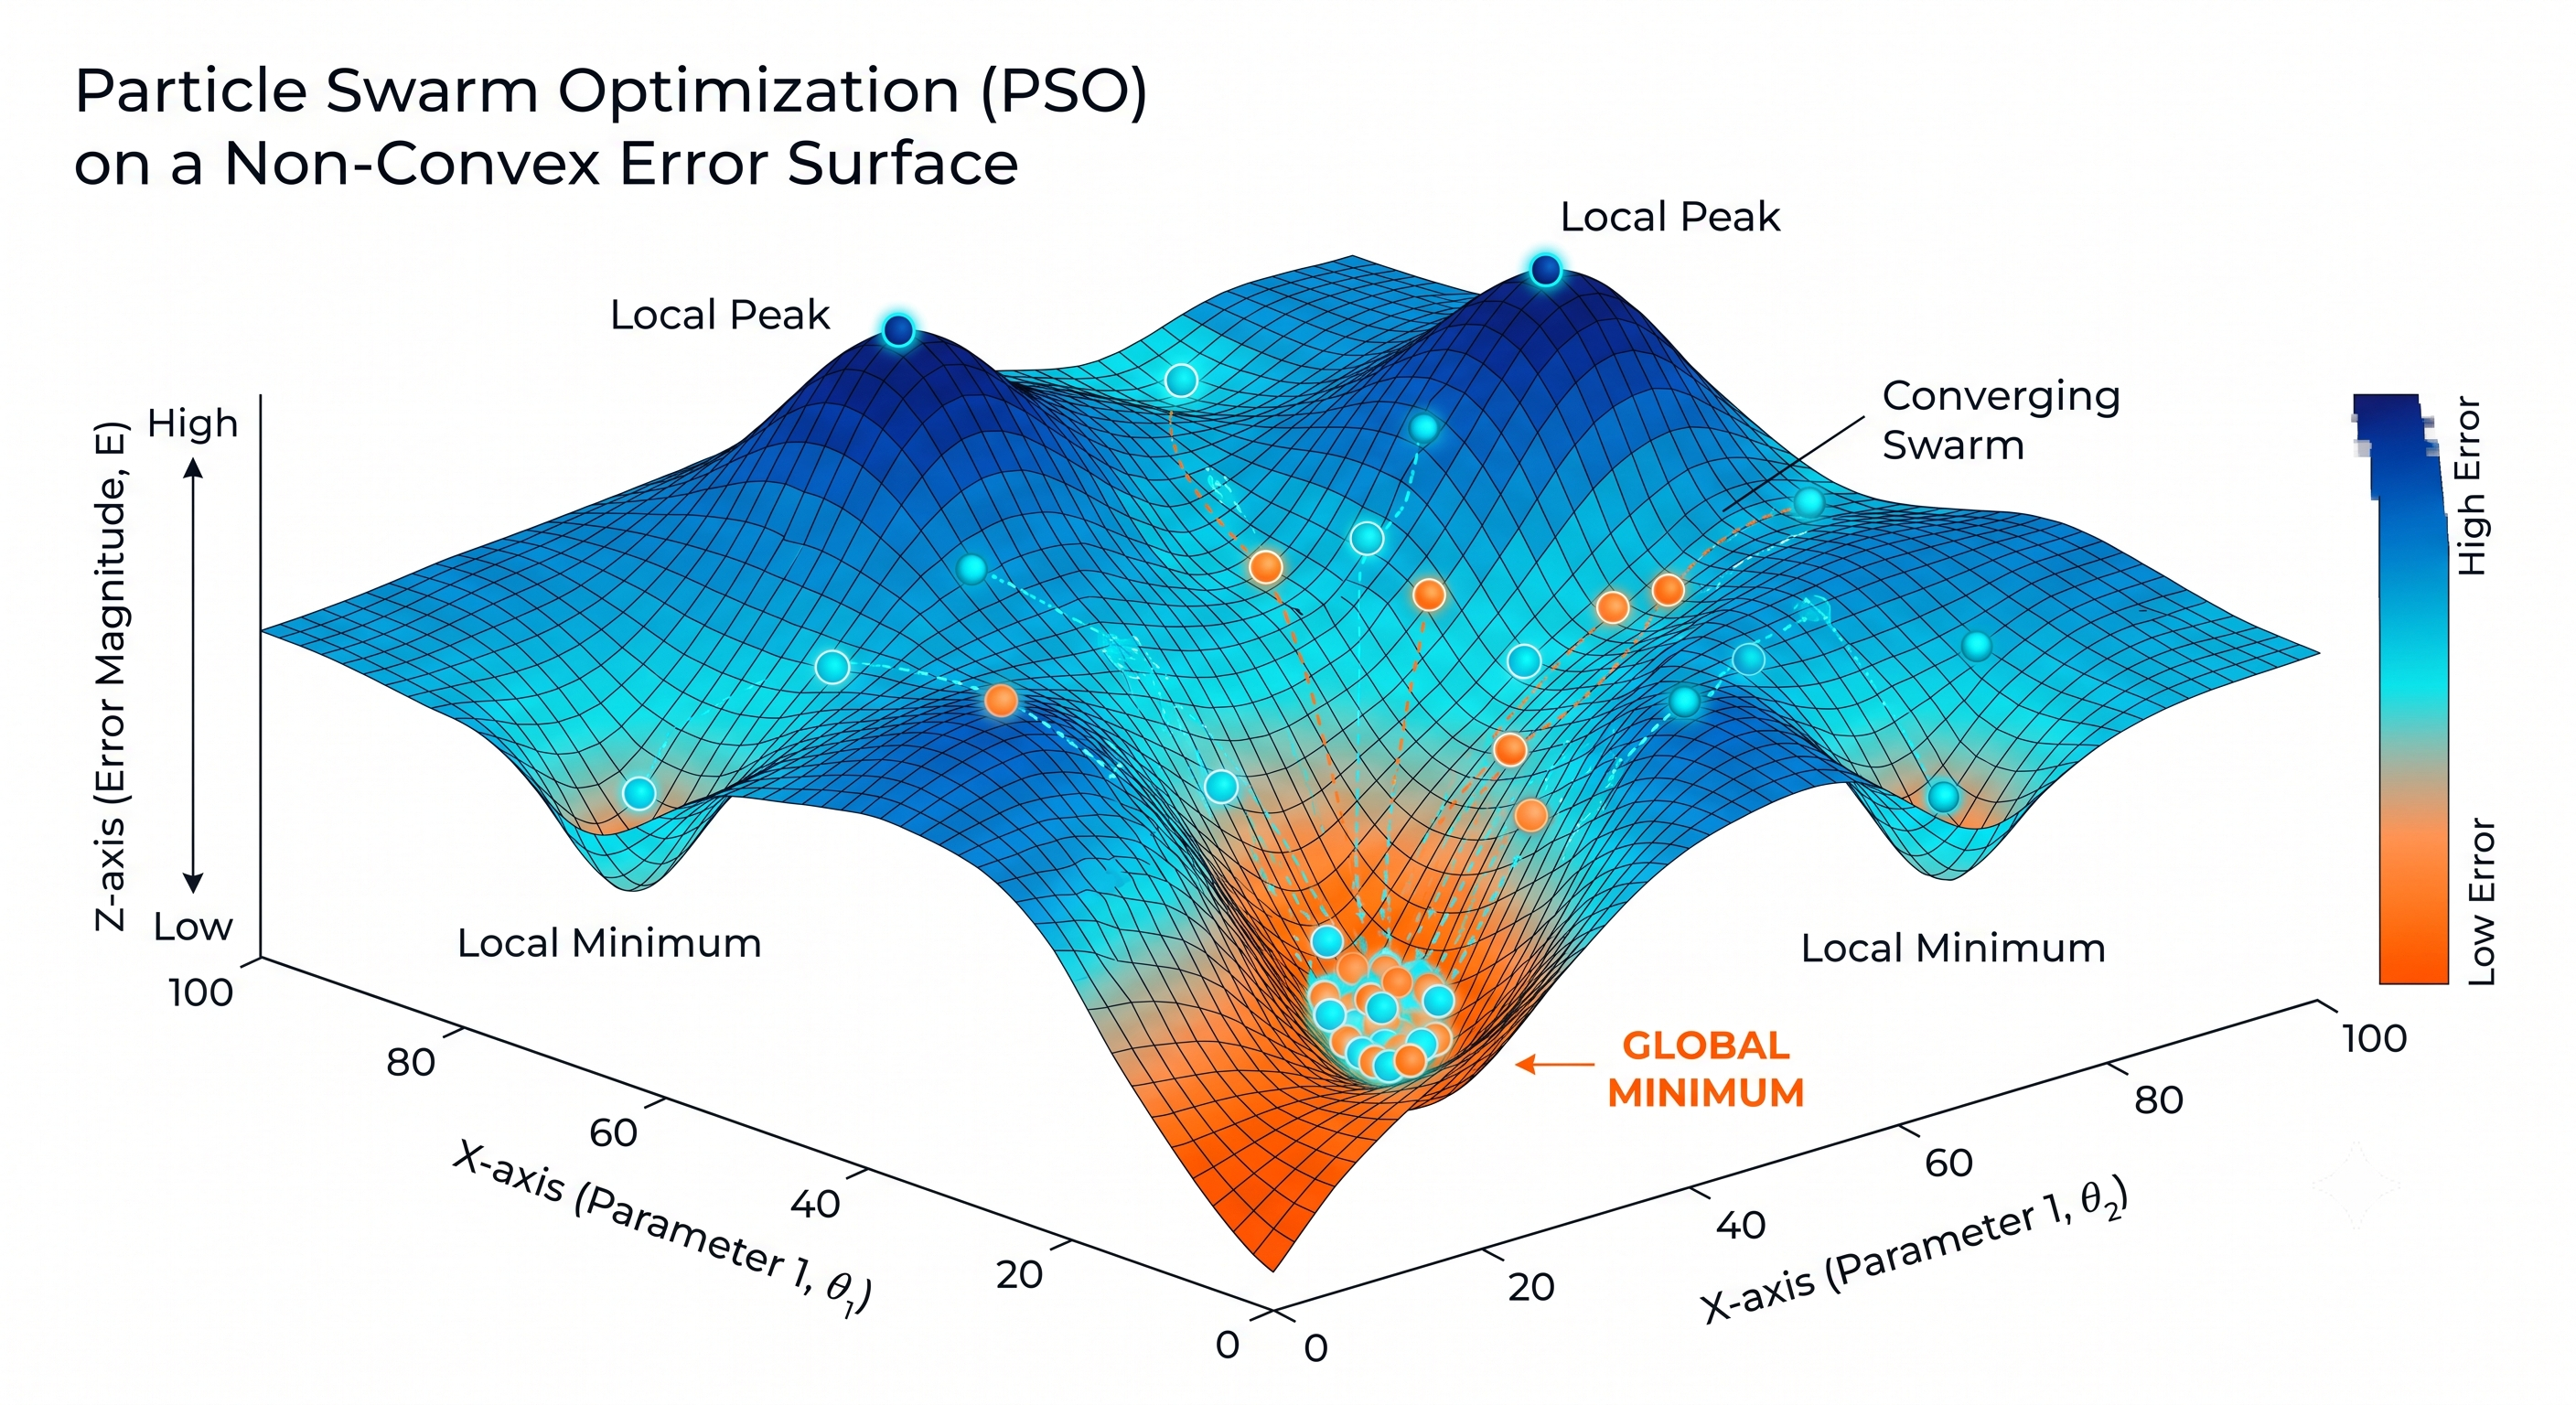
\includegraphics[width=0.65\textwidth]{Gemini_Generated_Image_y3pcuty3pcuty3pc.png}
\caption{Conceptual visualization of Particle Swarm Optimization (PSO). Particles navigate a complex, non-convex error surface to locate the global minimum parameter vector, avoiding convergence on local minima.}
\label{fig:pso_error_surface}
\end{figure}

To guarantee convergence without arbitrarily clamping the velocity, the constriction-factor formulation instead scales the entire velocity update:
\begin{equation}
\label{eq:pso_constriction_vel}
v_i(k+1) = \chi\Big[v_i(k) + c_1 r_1\big(p_{\mathrm{best},i} - x_i(k)\big) + c_2 r_2\big(g_{\mathrm{best}} - x_i(k)\big)\Big],
\end{equation}
where $\chi \approx 0.7298$ in standard configurations. Absorbing-wall boundary conditions are also enforced so that candidate parameters cannot drift outside physically meaningful limits.

\section{Summary}
\label{sec:summary_ch4}

This chapter detailed the transition from continuous-time ECMs to discrete ARX formulations suitable for closed-form OLS identification, and showed how the statistical limitations of OLS are addressed by WLS. For non-convex, multi-exponential datasets, gradient-based refinement (LM) and heuristic global optimizers (GA, PSO) were introduced as complementary tools when a closed-form solution is unavailable or the error surface has multiple minima. Having established how to extract optimal baseline parameters offline, Chapter 5 introduces the adaptive filtering techniques needed to track these parameters in real time as they drift during operation.